\section{FPGA development process overview}

\subsection{FPGA generic design flow}
FPGA generic design flow is shown in the \figref{FPGAGenFlow}.

\begin{figure}[H]
	\begin{center}
		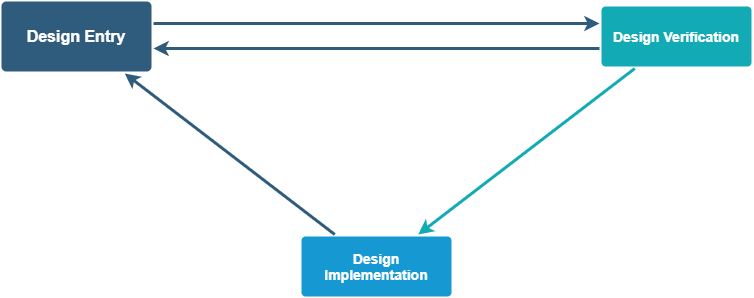
\includegraphics[width=\textwidth]{images/GenFlow.png}
		\caption{FPGA generic design flow}
		\label{FPGAGenFlow}
	\end{center}
\end{figure}

\subsubsection{Design Entry}
Creating design
Schematic / HDL Code

\subsubsection{Design Implementation}
Partitioning
Placing
Routing

\subsubsection{Design Verification}
Simulation for checking functionality
Debugging on the hardware: Logic Analyser




FPGA development process as shown in the \figref{FPGADevelopment} is usually divided in two parts: implementation and verification.

\begin{itemize}
	\item \textbf{Implementation} is the process of moving forward from your abstract design all the way to the final application. This is done by a tool chain of programs that perform a number of steps just like a compiler does. 
	\item \textbf{Verification} which is the necessary process of testing the design in every step of the implementation. And this is, as you may imagine, an iterative process. 
\end{itemize}	
	
\begin{figure}[H]
	\begin{center}
		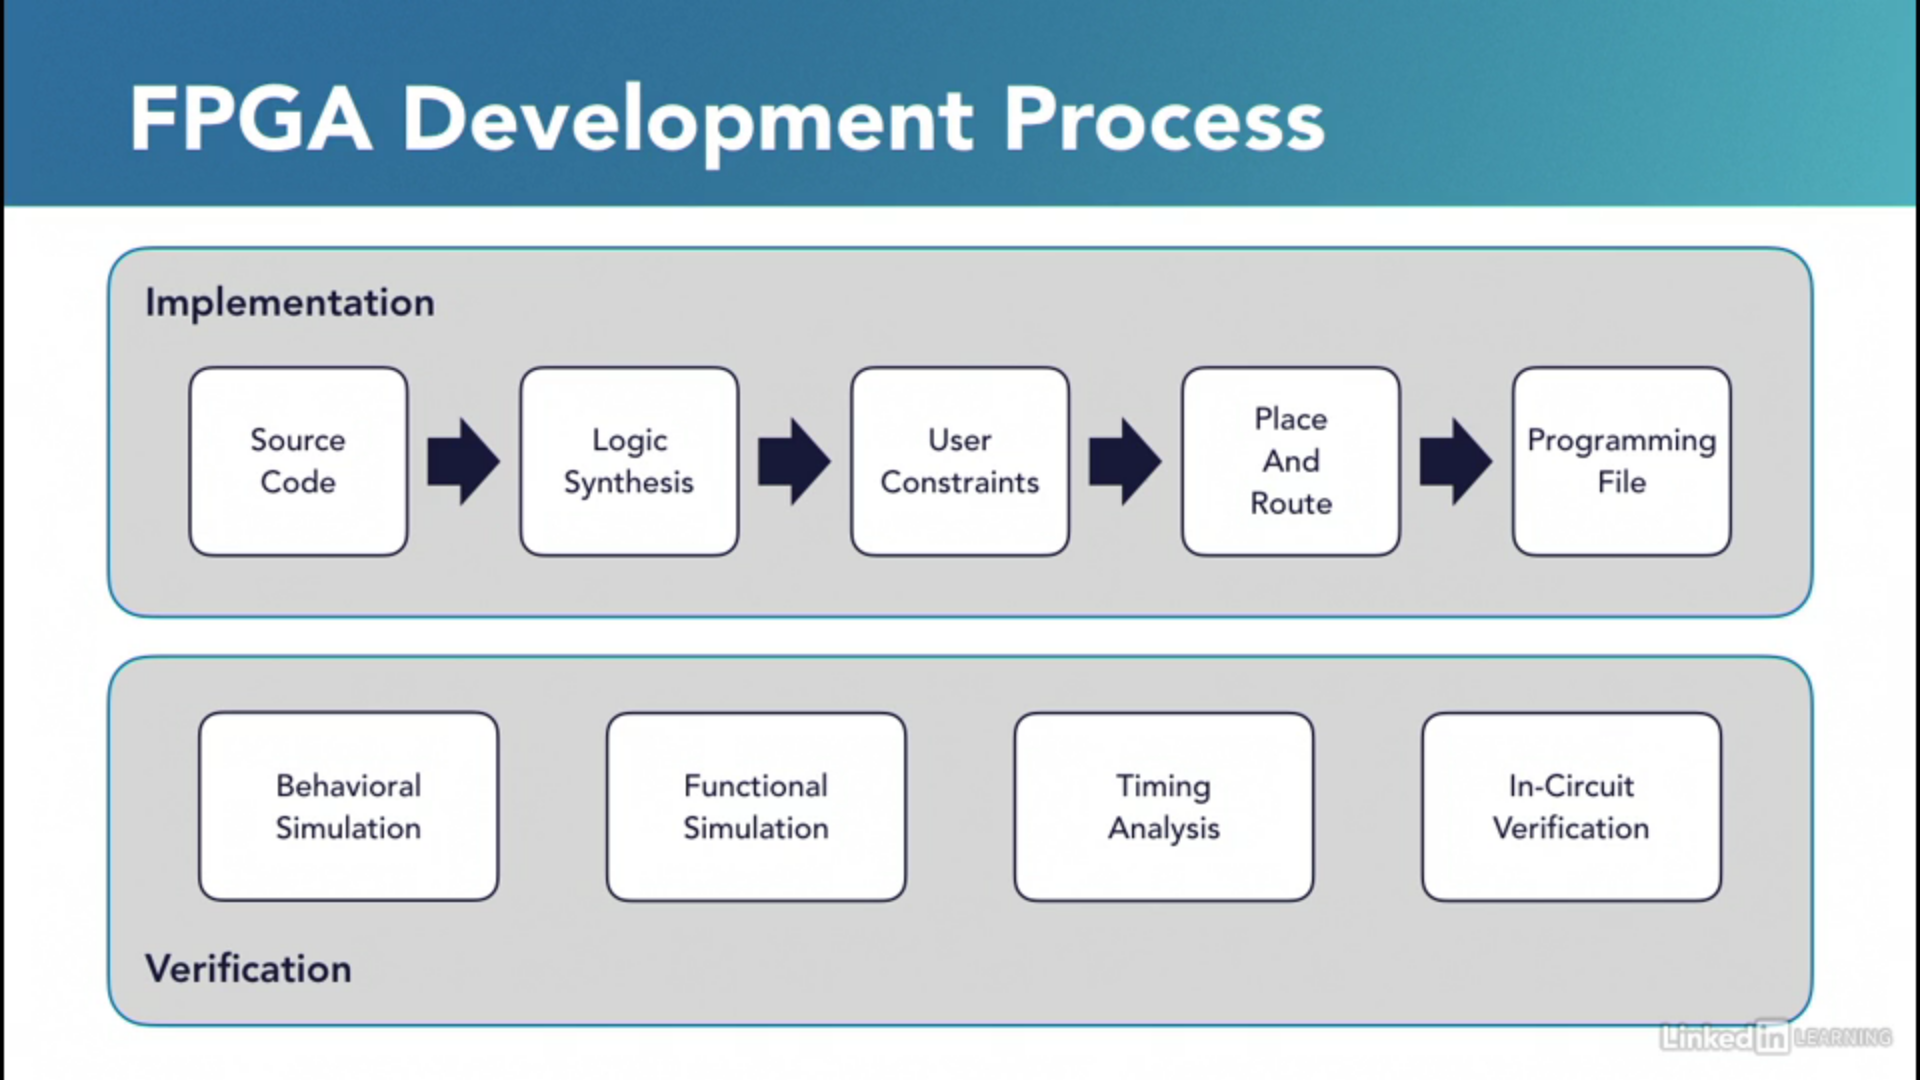
\includegraphics[width=\textwidth]{images/FPGADevelop.png}
		\caption{FPGA development process}
		\label{FPGADevelopment}
	\end{center}
\end{figure}

These are the steps involved in the implementation process. The first step is to write the source code which is a description of the hardware under development. There are several levels of abstraction to write this code. For example, your code can specify the connections in your system or the behavior of your system. This code is written in a hardware description language. The two most popular of which are VHDL and Verilog. Once the code is written, it goes through logic synthesis. A process very similar to software compiling. In fact, this whole process is sometimes called compiling. Logic synthesis consists in converting the source code into a net list that is a logic representation of the connections in the design under development. By this stage, not all HDL code is synthesizable. There are limitations in the FPGA's architecture that require your code to comply with some rules. A special level of abstraction known as the register transfer level or RTL is regarded as synthesizable most of the time. So it's very common to refer to the source code as RTL code. Once your design is understood by the tool chain, you get to specify the constraints of the final operational system. These are the requirements that you want the system to meet. The most important of these are timing constraints. You have to specify how fast you need your system to operate. When you inform the tool chain about your timing requirements, it can use these hints to choose a combination of connections that will produce the best system possible. Other aspects specified as user constraints are pin assignments, the area you want your design to occupy inside the chip, and the logic level voltages in the pins. Next the design goes through a process called place and route. This is where the net lists are translated into devices and connections, and these in turn are assigned to specific parts of the FPGA in what is known as a floor plan. Cells are assigned to logic elements, and the interconnects are routed. Finally you get to generate the programming file. The output of this stage is a binary file sometimes called a bit stream. The target may be an FPGA or some other memory. In fact, more often than not, FPGAs implement their internal configuration memory as volatile RAM. So there's usually an on board non-volatile memory with a boot up procedure that loads its content into the FPGAs configuration RAM. This whole process is prone to errors and bugs. So that's why the verification process is so important. There's at least one way to verify and validate your design at each step of the implementation. At the source code stage, you get to perform a behavioral simulation which reveals how the system behaves logically. After synthesis, a functional simulation can be performed which uses the newly produced gate level model. Once the timing constraints have been considered by the tool chain, a timing analysis can be performed to predict if there's any risk that your system will not meet these requirements, and the final application hardware can be put to the test with the help of in-circuit verification tools often provided by the FPGA vendor.

\begin{figure}[H]
\begin{center}
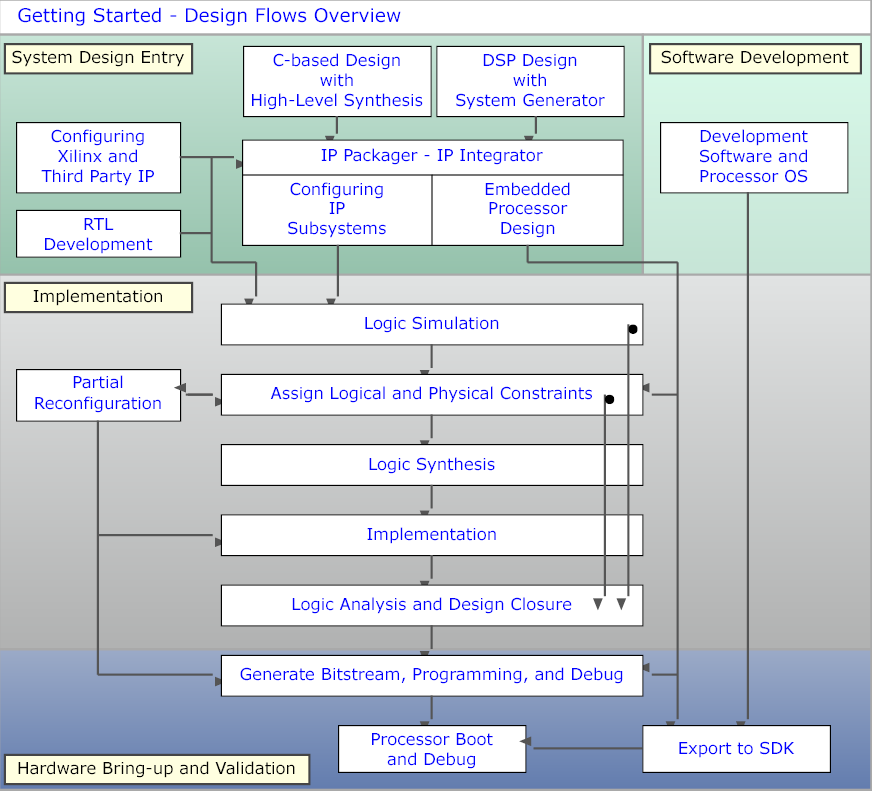
\includegraphics[width=\textwidth]{images/FPGADesignFlow.png}
\caption{Xilinx Vivado Workflow}
\label{VivadoOverview}
\end{center}
\end{figure}

The individual blocks Xilinx Vivado Workflow are explained below:

\subsection{RTL Design}
You can specify RTL source files to create a project and use these sources for RTL code development, analysis, synthesis and implementation. Xilinx supplies a library of recommended RTL and constraint templates to ensure RTL and XDC are formed optimally for use with the Vivado Design Suite. Vivado synthesis and implementation support multiple source file types, including Verilog, VHDL, SystemVerilog, and XDC.

\subsection{IP Design and System-Level Design Integration}
The Vivado Design Suite provides an environment to configure, implement, verify, and integrate IP as a standalone module or within the context of the system-level design. IP can include logic, embedded processors, digital signal processing (DSP) modules, or C-based DSP algorithm designs. Custom IP is packaged following IP-XACT protocol and then made available through the Vivado IP catalog. The IP catalog provides quick access to the IP for configuration, instantiation, and validation of IP. Xilinx IP utilizes the AXI4 interconnect standard to enable faster system-level integration. Existing IP can be used in the design either in RTL or netlist format.

\subsection{IP Subsystem Design}
The Vivado IP Integrator environment enables you to stitch together various IP into IP subsystems using the AMBA AXI4 interconnect protocol. You can interactively configure and connect IP using a block design style interface and easily connect entire interfaces by drawing DRC-correct connections similar to a schematic. Connecting the IP using standard interfaces saves time over traditional RTL-based connectivity. Connection automation is provided as well as a set of DRCs to ensure proper IP configuration and connectivity. These IP block designs are then validated, packaged, and treated as a single design source. Block designs can be used in a design project or shared among other projects. The IP Integrator environment is the main interface for embedded design and the Xilinx evaluation board interface.

\subsection{I/O and Clock Planning}
The Vivado IDE provides an I/O pin planning environment that enables I/O port assignment either onto specific device package pins or onto internal die pads, and provides tables to let you design and analyze package and I/O-related data. Memory interfaces can be assigned interactively into specific I/O banks for optimal data flow. You can analyze the device and design-related I/O data using the views and tables available in the Vivado pin planner. The tool also provides I/O DRC and simultaneous switching noise (SSN) analysis commands to validate your I/O assignments.

\subsection{Xilinx Platform Board Support}
In the Vivado Design Suite, you can select an existing Xilinx evaluation platform board as a target for your design. In the platform board flow, all of the IP interfaces implemented on the target board are exposed to enable quick selection and configuration of the IP used in your design. The resulting IP configuration parameters and physical board constraints, such as I/O standard and package pin constraints, are automatically assigned and proliferated throughout the flow. Connection automation enables quick connections to the selected IP. 

\subsubsection{Board Files}

\subsection{Synthesis}
Vivado synthesis performs a global, or top-down synthesis of the overall RTL design.
However, by default, the Vivado Design Suite uses an out-of-context (OOC), or bottom-up design flow to synthesize IP cores from the Xilinx IP Catalog and block designs from the Vivado IP integrator. You can also choose to synthesize specific modules of a hierarchical RTL design as OOC modules. This OOC flow lets you synthesize, implement, and analyze design modules of a hierarchical design, IP cores, or block designs, out of the context of, or independent from the top-level design. The OOC synthesized netlist is stored and used during top-level implementation to preserve results and reduce runtime. The OOC flow is an efficient technique for supporting hierarchical team design, synthesizing and
implementing IP and IP subsystems, and managing modules of large complex designs.

The Vivado Design Suite also supports the use of third-party synthesized netlists, including EDIF or structural Verilog. However, IP cores from the Vivado IP Catalog must be synthesized using Vivado synthesis, and are not supported for synthesis with a third-party synthesis tool.

Synthesis derives an optimized list of physical components and their interconnections called a netlist from the model of a digital system described in an HDL. Synthesis produces a database describing the elements and structure of a circuit. It specifies how to fabricate a phyical integrated circuit that implements in silicon the functionality described by design entry.

\subsection{Design Analysis and Simulation}
The Vivado Design Suite lets you analyze, verify, and modify the design at each stage of the design process. You can run design rule and design methodology checks, logic simulation, timing and power analysis to improve circuit performance. This analysis can be run after RTL elaboration, synthesis, and implementation. 

The Vivado simulator enables you to run behavioral and structural logic simulation of the design at different stages of the design flow. The simulator supports Verilog and VHDL mixed-mode simulation, and results can be displayed in a waveform viewer integrated in the Vivado IDE. You can also use third-party simulators that can be integrated into and launched from the Vivado IDE.

\subsubsection{Simulation}
 Logic debugging on PC before implementation of hardware. Allows line by line debug. Allows use of external files to simulate circuit. Testbench is another wrapper which tests the module you want to test (DUT: Device under test).

Functions only in the simulation(non synthesizable): 
\begin{itemize}
	\item \$monitor
	\item \$display
	\item \$stop
	\item \$finish
	\item \$error
\end{itemize}

clock generation:

\textit {always begin \\
	clk <= 1; \#5; \\
	clk <= 0; \#5; \\
	end;}
	

\subsection{Placement and Routing}
When the synthesized netlist is available, Vivado implementation provides all the features necessary to optimize, place and route the netlist onto the available device resources of the target part. Vivado implementation works to satisfy the logical, physical, and timing constraints of the design. For challenging designs the Vivado IDE also provides advanced floorplanning capabilities to help drive improved implementation results. These include the ability to constrain specific logic into a particular area, or manually placing specific design elements and fixing them for subsequent implementation runs. 

\subsection{Hardware Debug and Validation}
After implementation, the device can be programmed and then analyzed with the Vivado logic analyzer, or within the standalone Vivado Lab Edition environment. Debug signals can be identified in the RTL design, or inserted after synthesis and are processed throughout the flow. Debug cores can be configured and inserted either in RTL, in the synthesized netlist, or in the implemented design using incremental implementation techniques. Existing debug probes can be also modified, or internal signals routed to a package pin for external probing using the ECO flow. 

\subsection{Generate Bitstream}
\subsection{Program FPGA}
\subsection{FAQs}


\section{Vivado} 




\section{HDL} Hardware Description Language (HDL) is a specialized computer language used to describe the structure and behavior of electronic circuits, and most commonly, digital logic circuits.

A hardware description language enables a precise, formal description of an electronic circuit that allows for the automated analysis and simulation of an electronic circuit. It also allows for the synthesis of an HDL description into a netlist (a specification of physical electronic components and how they are connected together), which can then be placed and routed to produce the set of masks used to create an integrated circuit.

First, the purpose of an HDL is hardware entry for your toolchain to understand what system you want to produce. A simulator may be used to interpret your code in order to predict its behavior. And later a synthesis tool may be used to implement the design in a FPGA or ASIC. The built in structure of an HDL based project consists of two categories of modules. 

A. Descriptive modules, where you define your hardware and test bench or stimulus modules, where you enter a sequence of inputs to your system. 

B. Test bench modules are used by simulators to execute the steps you entered and produce the results you want to see.

In \figref{HDLCode} we have two code examples for the same module in Verilog and VHDL. The module is the one shown in the schematic diagram and it's a halfAdder, a basic block to implement a circuit that adds two integers. A halfAdder calculates the addition of a one bit number with another one bit number. If you look at the Verilog code at the left, you'll see that the syntax is somewhat similar to the C programming language. Modules are defined in a similar way to functions in C, but instead of a parameter list they have a port list because remember, this is a hardware module. Notice that this list specifies which port is an input and which port is an output. Next, the body of the module is just two lines of code which are instantiations of an and gate and an xor gate. Notice that the first wire specified is the output and the remaining ones are the inputs. Take your time to read the code and try to understand what it means. 

\begin{figure}[H]
	\begin{center}
		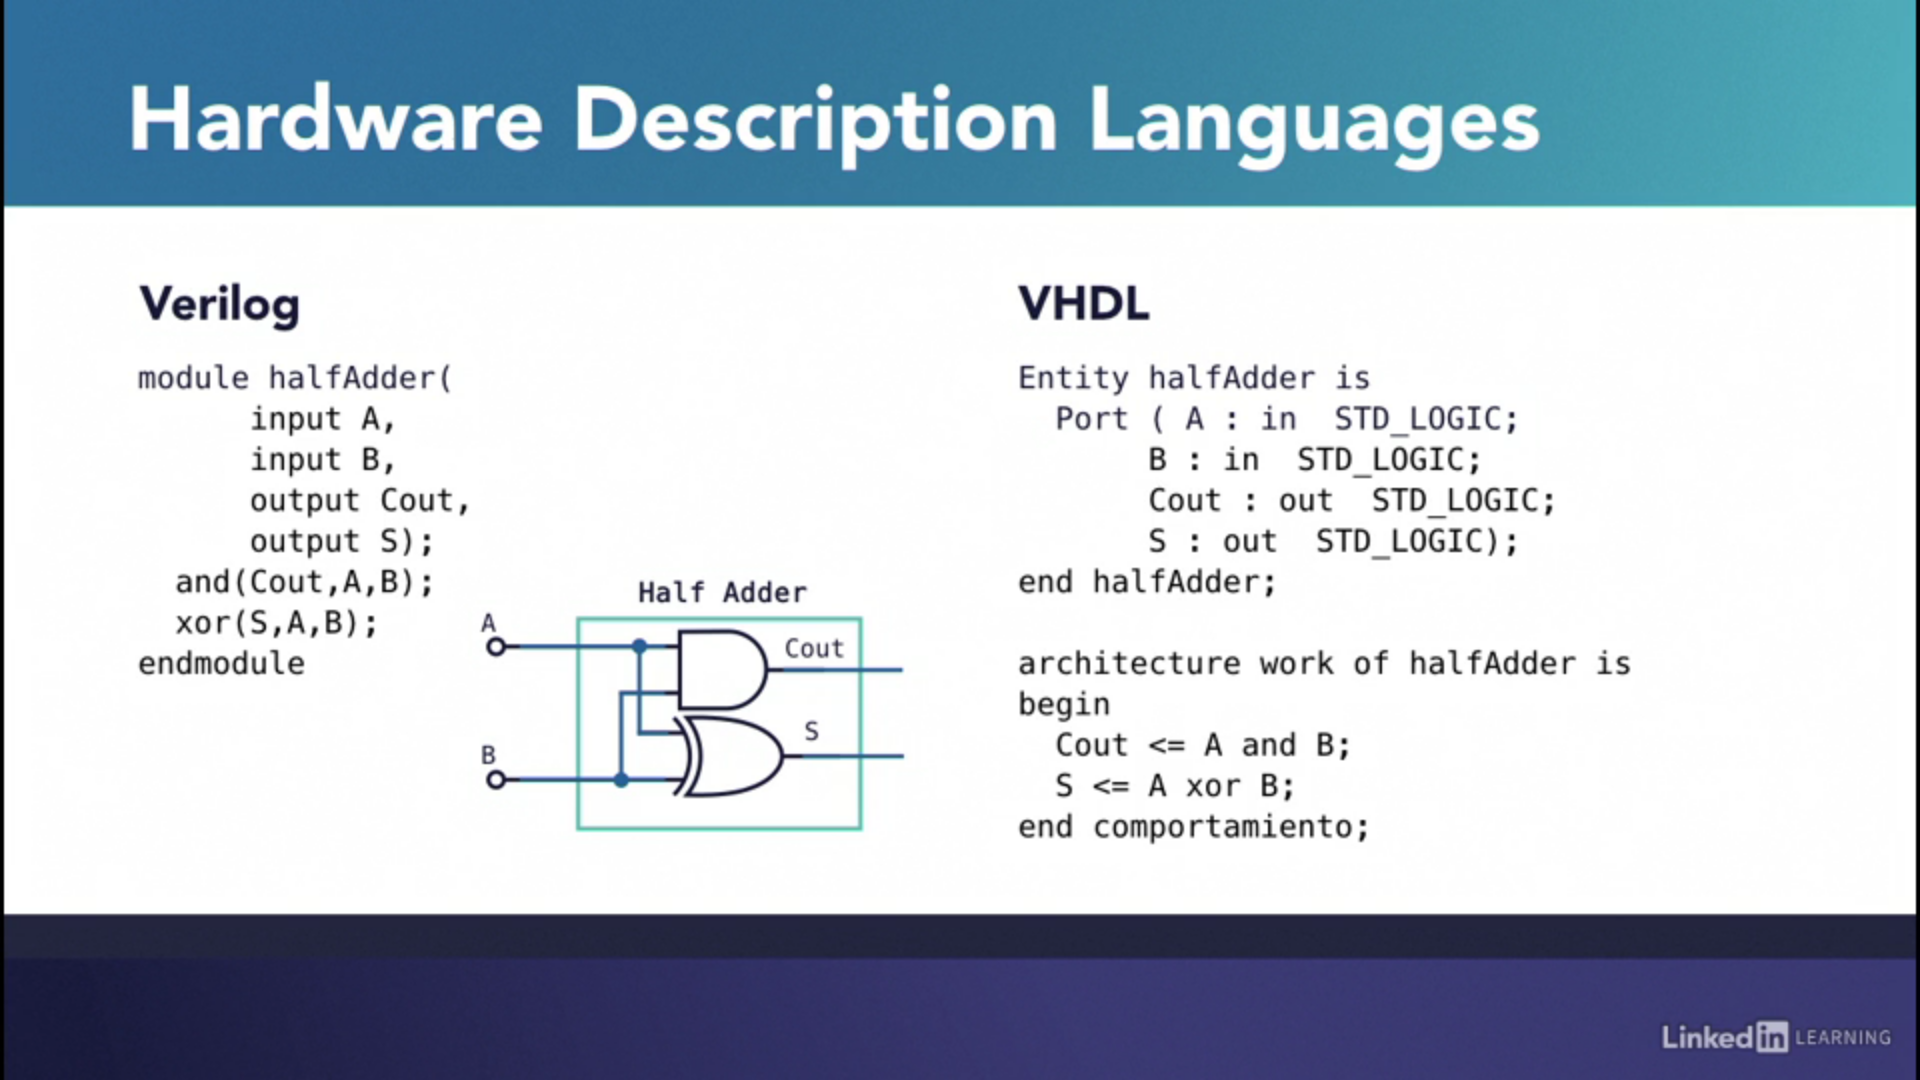
\includegraphics[width=5in]{images/HDL.png}
		\caption{HDL Code of Half Adder}
		\label{HDLCode}
	\end{center}
\end{figure}

At the right we have its equivalent in VHDL, which is a language inspired by the Ada and Pascal programming languages. In VHDL the port list is specified in what is known as an entity and the implementation is defined in an architecture. One can notice the differences and similarities between these languages.

\begin{figure}[H]
	\begin{center}
		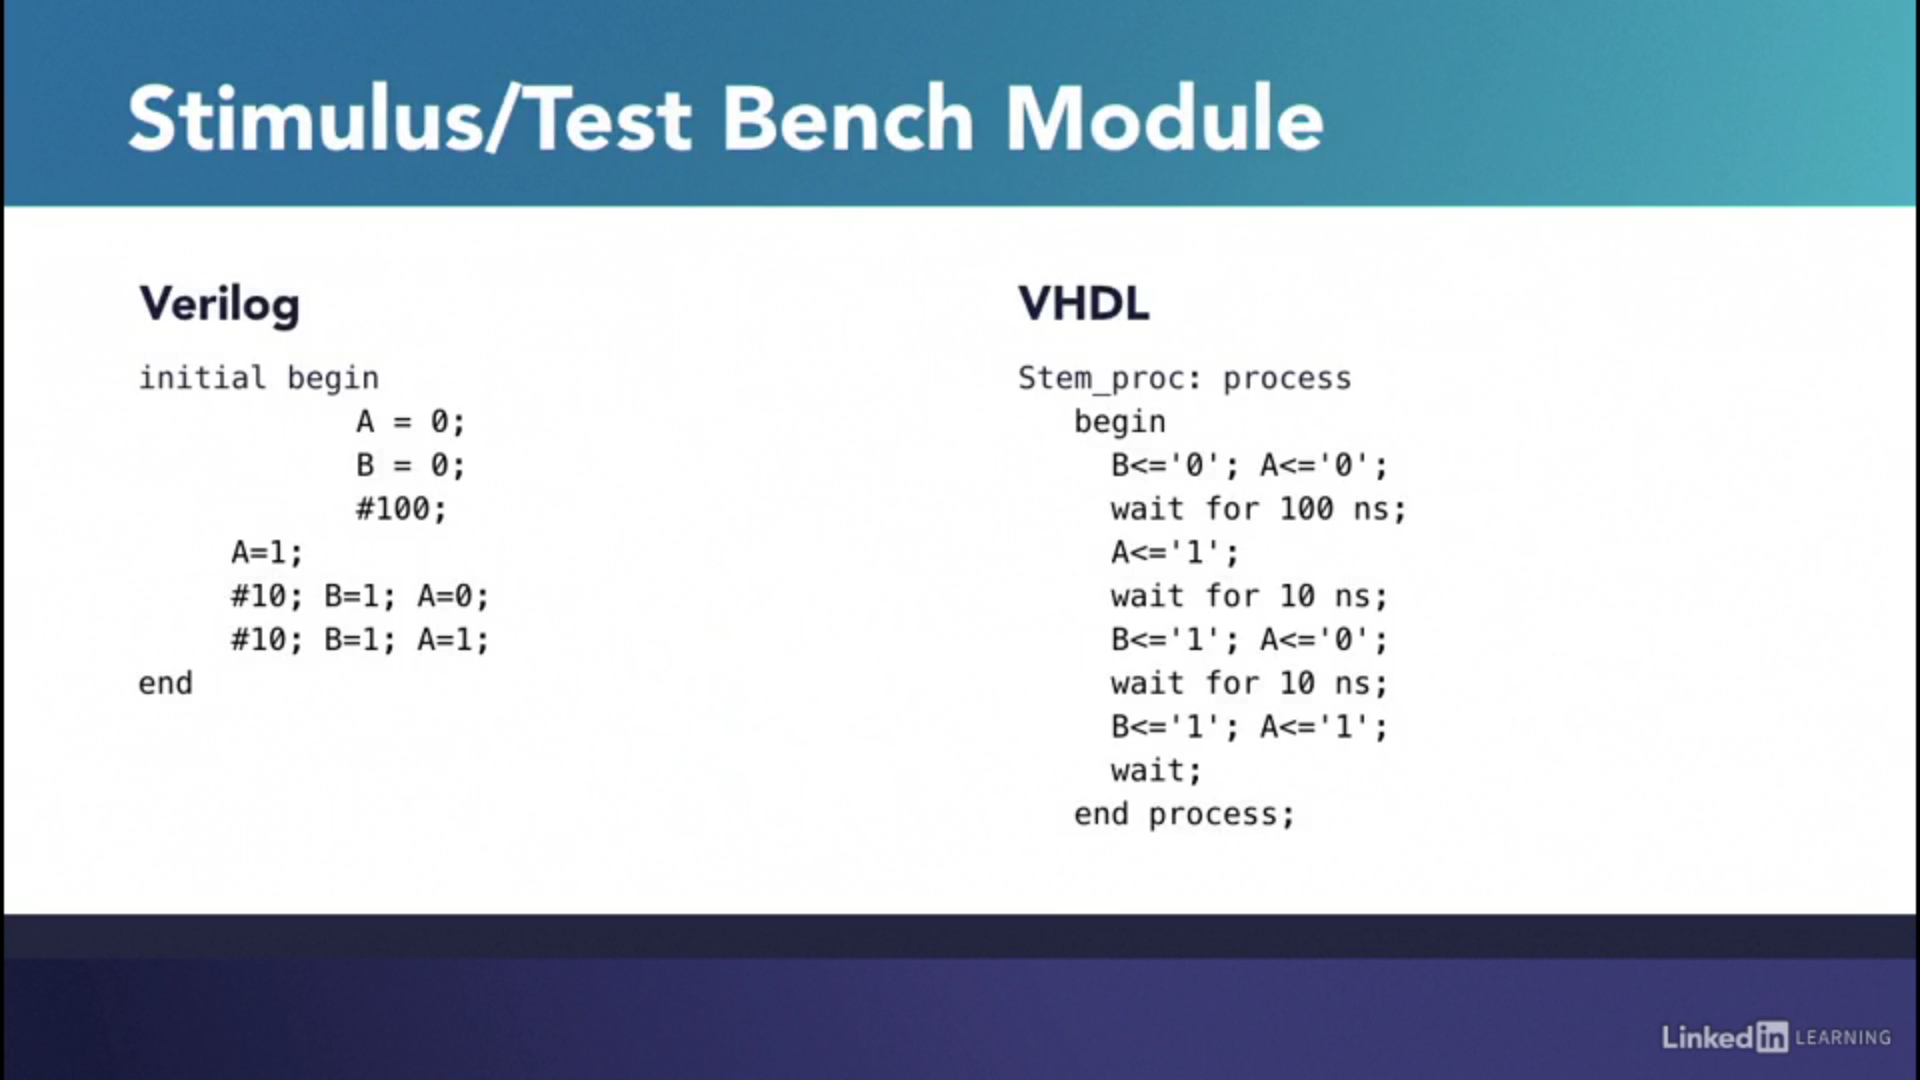
\includegraphics[width=5in]{images/HDLTB.png}
		\caption{HDL Testbenches of Half Adder}
		\label{HDLTB}
	\end{center}
\end{figure}

Finally, here's a partial test bench module in both languages describing the same course of events for a simulation. In this example we have two registers named A and B, which both take the value of zero. Then there's a 100 nanosecond pause before assigning one to A and then more assignments are performed on A and B separated by 10 nanosecond pauses. 

\subsection{Digital system modeling}
There are two main categories of digital systems. 
\begin{itemize}
	\item \textbf{Combinational logic}, where the signals travel from an input through the logic circuit, progressing forward with no feedback loops, all the way to the output. Combinational systems have no memory and thus no notion of time. Every combination of input values will always yield the same output. Examples of combinational circuits are multiplexers, de-multiplexers, and arithmetic Adders.
	\item \textbf{Sequential logic} has a combinational part with some feedback loops. This is the basic principle for flip flops, which are elements capable of holding a value acting as memory. This characteristic gives sequential systems a notion of time so they require a clock signal, which is a sequence of zeros and ones, at a constant known frequency. Examples of sequential systems are registers, counters, shift registers, and virtually every useful digital system, like a computer. 
\end{itemize}	

When it comes to modeling a digital system there are several levels of abstraction that you may use in your code to let the toolchain know what hardware you want to implement. 

\begin{itemize}
	\item Behavioral Model: A rather high level of abstraction is the behavioral model in which you tell the toolchain what your system is supposed to do, how it's supposed to behave. 
	
	\item Structural Model: There's also the structural model where you specify connections. Remember that you're designing hardware and so, multiple blocks will eventually be connected to each other. So in a structural model, you get to specify these connections. This the level you'll use when you instantiate modules.
	
	\item Gate-level Model: A lower level of abstraction is the gate level model which is very specific on the individual connections inside logic cells. This is similar to assembly language where most of the time you're advised to leave it to the compiler. 
	
\end{itemize}

Just like in traditional programming, these levels of abstraction are not mutually exclusive so you may have parts of your code at different levels if you need to. Hardware description languages were created to implement a modular design. So the modules you'll write are describing blocks of hardware, like a counter, a pre-scaler, an adder, or a decoder. These modules are instantiated as hardware building blocks, so a complete digital system is usually created by nesting these block instances. Now be aware that instantiating hardware blocks inside a loop makes no sense at all. You would be instructing the toolchain to dynamically spawn new hardware blocks. This is just not as safe as allocating memory in a program because you have no guarantees on how the new hardware will behave. So all hardware modules are rigid. They don't change dynamically.

\subsubsection{Levels of abstraction}
When writing a code in a hardware description language, one gets to express your digital systems in several levels of abstraction. In Verilog, there's a traditional distinction between the following levels. 

\begin{itemize}
	\item Gate level, also called as Structural level: The gate level is the assembly language of FPGAs. At this level, all of the connections and devices are explicitly described. The building blocks are single logic devices or gates. So at the gate level the code only contains wires and gates.
	\item Register-transfer level(RTL): The register-transfer level is the most widely-used level of abstraction, so much so that Verilog and VHDL code is often referred to as RTL code. The register-transfer level employs higher-level semantics than the gate level.
	\item Behavioral level: The behavioral level concentrates on the behavior of your system. The code is not always synthesizable, meaning that some parts of the code may be a little too ambiguous to successfully yield a physical FPGA or ASIC. This level contains elements to provide quick information to the development tools, often useful in simulations for validation and verification.
\end{itemize} 
	
These levels are not mutually exclusive. In fact, it's very uncommon to come across code that uses one level exclusively. Useful digital systems aren't exclusively written at the behavioral, register-transfer, or gate level. As one may presume, they may combine modules at different levels of abstraction. 


\subsection{Verilog}
Operator Precedence:
The order of the table tells what operation is made first, the first ones has the highest priority. The () can be used to override default. 
\subsubsection{Features of Verilog}
\begin{itemize}
	\item Case sensitive
	\item All keywords are lowercase
	\item Semicolon is the statement terminator
	\item //: single line comment
	\item /* */: multiline comment
\end{itemize} 


\subsubsection{Verilog Code structure}
Sample code to explain verilog code structure:
    \begin{lstlisting}[style={verilog-style}]
        // timescale directive tells the simulator the base units and precision of the simulation 
        `timescale 1 ns / 10 ps 
        module name (input and outputs); 
        // parameter declarations 
        parameter parameter_name = parameter value; 
        // Input output declarations 
        input in1; 
        input in2; // single bit inputs 
        output [msb:lsb] out; // a bus output 
        // internal signal register type declaration - register types (only assigned within always statements). reg register
        variable 1; 
        reg [msb:lsb] register variable 2; 
        // internal signal. net type declaration - (only assigned outside always statements) wire net variable 1; 
        // hierarchy - instantiating another module 
        reference name instance name ( 
        .pin1 (net1), 
        .pin2 (net2), 
        . 
        .pinn (netn) 
        ); 
        // synchronous procedures 
        always @ (posedge clock) 
        begin 
        . 
        end 
        // combinatinal procedures 
        always @ (signal1 or signal2 or signal3) 
        begin 
        . 
        end 
        assign net variable = combinational logic; 
        endmodule 
    \end{lstlisting}
  
Types of elements in Verilog are Wires and Registers.
\begin{itemize}
	\item \textbf{Wires} make connections between elements. They implement nets. Otherwise known as nodes in the circuit. Since wires are simply nets. They are driven by signals. They may not always have a value. So, they may have a high impedance or High-Z state. Which is neither a zero or one. But, equivalent to a floating node. 
	\item \textbf{Registers} can also make connections between elements in the code. But, registers can be a assign values. And they hold those values until the next assignment. And finally registers can drive wires. 
\end{itemize} 
	
Just a quick warning! The name register is misleading. Because Verilog registers do not necessary produce Flip flops in a FPGA or ASIC implementation. The synthesis tool will decide if the behavior really requires and actual register.


\subsubsection{Net data types}
\begin{itemize}
	\item wire: represents a node or connection
	\item tri: represents a tri-state node
	\item supply0: constant logic 0
	\item supply1: constant logic 1
\end{itemize} 

\subsubsection{Variable data types}
\begin{itemize}
	\item reg: unsigned variable of any bit size (reg signed : signed implementation)
	\item integer: signed 32-bit variable
	\item real,time,realtime: non-synthesizable
\end{itemize} 

\subsubsection{Two methods to define port connections}
\begin{itemize}
	\item By ordered list: port connections defined by the order of the port list in the lower-level module.
	\item By name: port connections defined by name, order of the port connections does not matter.
	\item Mixed is not possible.
\end{itemize} 

Parameter is value assigned to a symbolic name.
localparam is same as parameter but cannot be overwritten.


\clearpage
\subsubsection{Operators}
Verilog operators operate on several data types to produce an output. Not all Verilog operators are synthesible (can produce gates). Some operators are similar to those in the C language. Remember, you are making gates, not an algorithm (in most cases).

\begin{table}[H]
\begin{center}
\begin{tabular}{@{}lll@{}}
\toprule
\textbf{Character}                 & \textbf{Operation}             & \textbf{Type of operator}  \\ \midrule
+                                  & Add                            & Arithmatic   \\
-                                  & Subtract                       & Arithmatic   \\
/                                  & Divide                         & Arithmatic   \\
*                                  & Multiply                       & Arithmatic   \\
\%                                 & Modulus                        & Arithmatic   \\
$\sim$                             & Invert                         & bitwise      \\
\&                                 & And                            & bitwise      \\
|                                  & Or                             & bitwise      \\
$\wedge$                           & Xor                            & bitwise      \\
$\wedge$$\sim$  or $\sim$$\wedge$  & Xnor                           & bitwise      \\
\&	                               & And all bits                   & reduction    \\
$\sim$ \&	                       & Nand all bits                  & reduction    \\
|                                  & Or all bits                    & reduction    \\
$\sim$ |                           & Nor all bits                   & reduction    \\
$\wedge$                           & Xor all bits                   & reduction    \\
$\wedge$  or $\sim$$\wedge$        & Xnor all bits                  & reduction    \\
>	                               & Greater than                   & Relational   \\
<	                               & Smaller than                   & Relational   \\
>=	                               & Greater than or equal          & Relational   \\
<=	                               & Smaller than or equal          & Relational   \\
==	                               & Equality                       & Relational   \\
!=	                               & Inequality                     & Relational   \\
===	                               & Case equality                  & Relational   \\
!===	                           & Case inequality                & Relational   \\
!                                  & Not true                       & Logical      \\
\&\&                               & Both expressions true          & Logical      \\
||                                 & One or both expressions true   & Logical      \\
>>                                 & Shift right                    & shift        \\
<<                                 & Shift left                     & shift        \\
?                                  & Conditions testing             & Misc         \\
\{\}                               & Concatenate                    & Misc         \\
\{\{\}\}                           & Replicate                      & Misc         \\ \bottomrule
\end{tabular}
\end{center}
\end{table}
\clearpage


Operator Precedence:
The order of the table tells what operation is made first, the first ones has the highest priority. The () can be used to override default. 
\begin{figure}[H]
	\begin{center}
		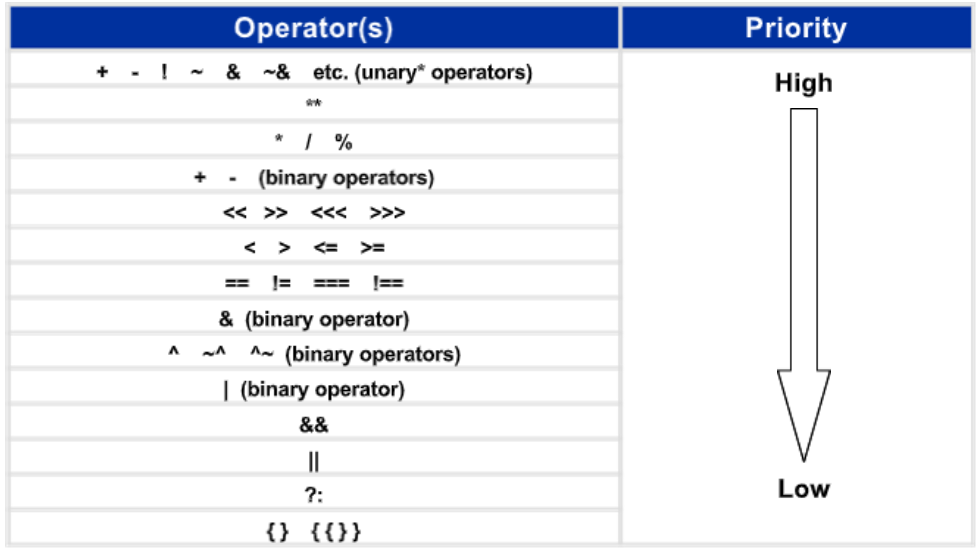
\includegraphics[width=5in]{images/OperatorPrecedence.png}
		\caption{Operator Precedence}
		\label{OperatorPrecedence}
	\end{center}
\end{figure}


\subsubsection{Assignments}
Assignment statements are categorized as follows:
\begin{description}
\item[Continuous assignments] Model the behavior of combinational logic by using expressions and operators. 
Always active: LHS is updated upon RHS changes
LHS must be a net data type.
RHS can be a bet, register or function calls.
Delay values can be assigned to model gate delays.


\item[Procedural assignments] Procedural assignments are made inside procedural blocks such as:\\
i. initial: Initializes behavioral statements for simulation. Initial block starts at 0, executes only once during simulation, and then does not execute again.\\
ii. always: Descibe the circuit functionality using behavioral statements. Block executes concurrently starting at time 0 and continuously in a looping fashion.

\par Each always and initial block represents a separate process. Processes run in parallel and start at simulation time 0. Statements inside a process execute sequentially. always and inital blocks cannot be nested.

Two types of procedural assignents:
\begin{itemize}
    \item Blocking assignments: executed in the order they are specified in a sequential block
    \item Non blocking assignments: Allow scheduling of assignments without blocking execution of  the statements that follow in a sequential block.
\end{itemize}

\end{description}

\subsubsection{RTL processes}
There are two types of RTL processes:
\begin{itemize}
    \item Combinatorial Process: sensitive to all inputs used in the combinatorial logic. ex: always @(a,b,sel)
    \item Clocked proess: sensitive to a clock or/and control signal. ex: always @(posedge clk, posedge rst)
\end{itemize}

\subsubsection{Behavioral statements}

Must be inside a procedural block (initial or always)

\begin{description}
\item[if-else] conditions are evaluated in order from top to bottom, Prioritization
\item[case] conditions are evaulated at once, No prioritization
\item[Loop] used for repetitive operations.
\begin{itemize}
    \item forever: infinite loop, non synthesizable
    \item repeat: executes a fixed number of times
    \item while: repeates until condition is achieved, non synthesizable
    \item for: executes initial assignment at the start of the loop and then executes loop body if expression is true.
\end{itemize}

\end{description}


\subsubsection{Subprograms}
Defined within a module. Uses: replacing repititive code, enhancing readability.

\begin{description}
\item[Functions] return a value based on its inputs, produces combinational logic. Always execute in zero time. Cannot pause their execution. Cannot contain delay, event, or timing control statements. Must have at least one input argument. Arguments may not be outputs, or inouts. Always return a single value. Ex: assign multOut = mult(ina, inb)

\item[Tasks] Like procedures in other languages, can be combinatorial or registered. May execute in non-zero simulation time. May contain delay, event, or timing control statements. May have zero or more input, output, or inout arguments. Ex: stmOut(nxt, first, sel, filter)

\begin{figure}[H]
	\begin{center}
		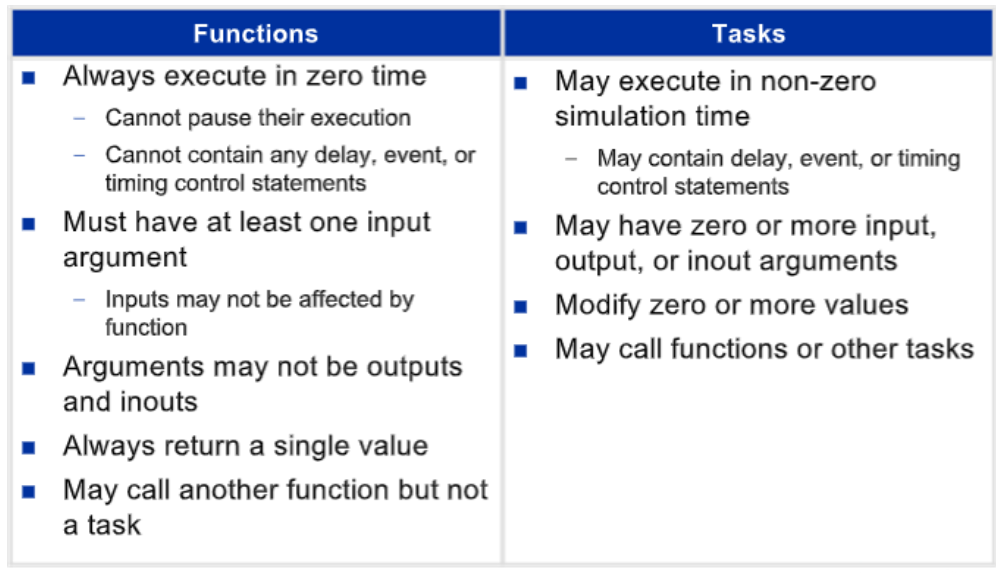
\includegraphics[width=5in]{images/VerilogFuncTasks.png}
		\caption{Verilog Functions and Tasks}
		\label{VerilogFuncTasks}
	\end{center}
\end{figure}


\end{description}

\iffalse
\subsection{Verilog}
Types of elements in Verilog are Wires and Registers.
\begin{itemize}
	\item \textbf{Wires} make connections between elements. They implement nets. Otherwise known as nodes in the circuit. Since wires are simply nets. They are driven by signals. They may not always have a value. So, they may have a high impedance or High-Z state. Which is neither a zero or one. But, equivalent to a floating node. 
	\item \textbf{Registers} can also make connections between elements in the code. But, registers can be a assign values. And they hold those values until the next assignment. And finally registers can drive wires. 
\end{itemize} 
	
Just a quick warning! The name register is misleading. Because Verilog registers do not necessary produce Flip flops in a FPGA or ASIC implementation. The synthesis tool will decide if the behavior really requires and actual register.
\fi

\subsection{Verilog vs SystemVerilog} 

System Verilog and verilog both Both are IEEE standards, Verilog is IEEE 1364 -2005 (Latest Version)and System verilog is IEEE 1800 - 2017( Latest version). Verilog is a Hardware Description Language , whereas System verilog is a combination of Hardware Description Language (HDL) and Hardware Verification Language (HVL). So, System verilog can be considered as an extension or a superset of Verilog.

	
\begin{itemize}

    \item \textbf{History}\\ Verilog, is the popular Hardware Description Language invented in early 1980’s. Whereas, System Verilog started initially with a name, as Superlog in 2002 and was standardized in 2005 with its own name.\\
	System verilog for RTL design is an extension of verilog (2005) and has all of its features.System verilog for verification uses Object-oriented programming techniques.

	\item \textbf{Data types} Verilog has majorly two datatypes – Reg and Wire  which are 4 valued logic 0,1,x,z. Whereas, System verilog has logic(inclusive of Wire \& Reg),  int, shortint, longint, logic, bit, real, realtime, reg, chandle, user defined data type, etc. which are both combination of 4 and 2 valued logic.
	
	\item \textbf{Memory}Verilog does not allow packed array concept and the lifetime of memories will be static. Whereas, System verilog allows packed array declaration and the lifetime of memories can be dynamic.

	\item \textbf{Procedural Block} Verilog has a general purpose always block to model different types of hardware structures. Whereas, System verilog uses three different procedural blocks namely, always\_comb , always\_ff and always\_latch intended to model specific type of hardware description.

	\item \textbf{Construction} Verilog design is based on hierarchy of modules, where modules encapsulate the design hierarchy, and communicate with other modules through ports. Whereas , System verilog uses Class based design.

	\item \textbf{Interface} Verilog ports (larger designs) for describing a module’s connectivity with other module is difficult. Whereas, System verilog uses interface to reduce the redundancy of port declarations between modules.

	\item \textbf{Random} Verilog uses inbuit system functions like \$random and \$urandom, whereas System Verilog uses a method called Randomize().

	\item \textbf{Constraints} Verilog does not support any control over the variable to be randomized,Whereas System verilog uses constraints to have a control of what is being randomized.

	\item \textbf{TB Environment} Verilog does not support for having reusable testbenches and so for complex designs verification will be a milestone.Whereas, System verilog supports for having reusable testbenches.
	
	\item \textbf{Synchronisation} SystemVerilog uses interface construct which has used for bunching of all the signals along with clocking block which is used for synchronisation unlike Verilog in which instantiation with the DUT becomes tedious because of large number of signals.
	
\end{itemize}
\pagebreak



\section{Petalinux}
PetaLinux is a free Xilinx tool which offers everything necessary to customize, build and deploy Embedded Linux solutions on Xilinx processing systems. It enables developers to configure, build and deploy essential open source and systems software to Xilinx silicon, including: 
\begin{itemize}
  \item FSBL
  \item U-Boot
  \item ARM Trusted Firmware
  \item Linux
  \item Libraries and applications
\end{itemize}

With this tool developers can customize the boot loader, Linux kernel, or Linux applications. They can add new kernels, device drivers, applications, libraries, and boot \& test software stacks on the included full system simulator (QEMU) or on physical hardware via network or JTAG. Some features of Petalinux include:

\begin{enumerate}
  \item \textbf{Custom BSP Generation Tools} PetaLinux tools will automatically generate a custom, Linux Board Support Package including device drivers for Xilinx embedded processing IP cores, kernel and boot loader configurations.
  \item \textbf{Linux Configuration Tools} PetaLinux includes tools to customize the boot loader, Linux kernel, file system, libraries and system parameters.
  \item \textbf{Software Development Tools} PetaLinux tools integrate development templates that allow software teams to create custom device drivers, applications, libraries and BSP configurations.
  \item \textbf{Reference Linux Distribution} PetaLinux provides a complete, reference Linux distribution that has been integrated and tested for Xilinx devices. The reference Linux distribution includes both binary and source Linux packages including:
  \begin{itemize}
    \item Boot loader
    \item CPU optimized kernel
    \item Linux applications \& libraries
    \item C \& C++ application development
    \item Debug
    \item Thread and FPU support
    \item Integrated web server for easy remote management of network and firmware configurations
  \end{itemize}
\end{enumerate}

\clearpage
There are seven independent tools that make up the PetaLinux design flow. 
\begin{enumerate}
  \item \textbf{petalinux-create} tool either creates a new PetaLinux project directory structure or a component within the specified project.
  \item \textbf{petalinux-config} tool allows you to customize the specified project. Either a project is initialized or updated to reflect the specified hardware configuration or a specified component is customized using a menuconfig interface.
  \item \textbf{petalinux-build} tool builds either the entire embedded Linux system or a specified component of the Linux system. This tool uses the Yocto Project underneath. Whenever petalinux-build is invoked, it internally calls bitbake.
  \item \textbf{petalinux-boot} command boots MicroBlaze CPU, Zynq and Zynq UltraScale devices with PetaLinux images through JTAG/QEMU. With JTAG, images are downloaded and booted on a physical board using a JTAG cable connection. With QEMU, images are loaded and booted using QEMU, the software emulator.
  \item \textbf{petalinux-package} tool packages a PetaLinux project into a format suitable for deployment. Based on the target package format, the supported formats/workflows are boot(.BIN or .MCS), bsp, and pre-built.
  \item \textbf{petalinux-util} tool provides various support services to the other PetaLinux workflows.
  \item \textbf{petalinux-upgrade} PetaLinux tool has system software components (embedded SW, ATF, Linux, U-Boot, OpenAMP, and Yocto framework) and host tool components (Vivado Design Suite, Xilinx Software Development Kit (SDK), HSI, and more). To upgrade to the latest system software components, you must install the corresponding host tools (Vivado design tools). The petalinux-upgrade command resolves this issue by upgrading the system software components without changing the host tool components. 
\end{enumerate}

\subsection{Petalinux Design Flow}
\begin{enumerate}
  \item \textbf{Hardware platform creation} Vivado Design Suite
  \item \textbf{Create PetaLinux project} petalinux-create -t project
  \item \textbf{Initialize PetaLinux project} petalinux-config --get-hw-description
  \item \textbf{Configure system-level options} petalinux-config
  \item \textbf{Create user components} petalinux-create -t COMPONENT
  \item \textbf{Configure the Linux kernel} petalinux-config -c kernel
  \item \textbf{Configure the root file system} petalinux-config -c rootfs
  \item \textbf{Build the system} petalinux-build
  \item \textbf{Test the system on qemu} petalinux-boot --qemu
  \item \textbf{Deploy the system} petalinux-package --boot
  \item \textbf{Update the PetaLinux tool system software components} petalinux-upgrade --url/--file
\end{enumerate}

\clearpage
\subsection{QEMU} 
QEMU (Quick EMUlator) is an open source, cross-platform, system emulator. It is an executable that runs on an x86 Linux or Windows operating systems. QEMU can emulate a full system (commonly referred to as the guest), such as a Xilinx development boards. The emulation includes the processors, peripherals, and other hardware on the development board; allowing one to launch an operating system or other applications on the virtualized hardware. These applications can be developed using the exact same toolchain that would be used on physical hardware. QEMU can also interact with the host machine through interfaces, such as CAN, Ethernet and USB; allowing real-world data from the host to be used in the guest machine in real time.

\par Reasons why QEMU is used as an emulator and testing tool:
\begin{itemize}
  \item Remote Development
  \item Easier Debugging
  \item Easier Testing
  \item Developing and Running an OS
  \item Hardware Modeling and Verification
  \item Safety and Security
\end{itemize}

QEMU works by using dynamic translation. Instructions are translated from the guest's instruction set to the equivalent host machine instructions. The equivalent host instructions are then executed on the host, and the results of those instructions are then pushed back into the guest machine.
    
\begin{figure}[H]
\begin{center}
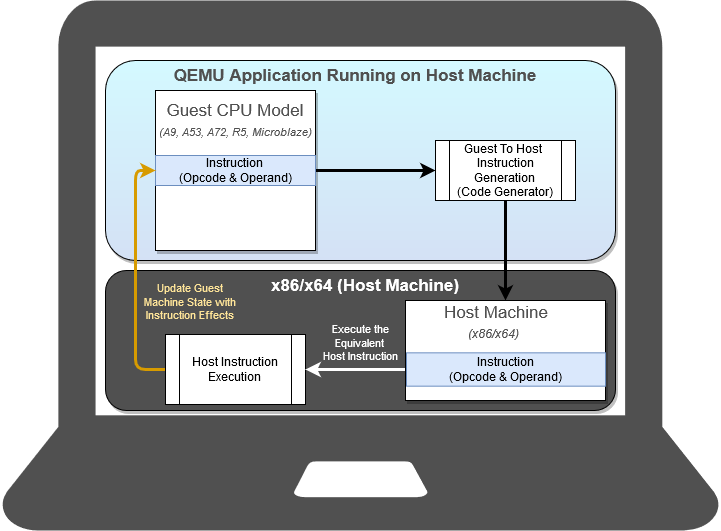
\includegraphics[width=\textwidth]{images/QEMU.png}
\caption{QEMU Functionality}
\label{QEMU}
\end{center}
\end{figure}

\pagebreak


\section{Version Control: Git, Bitbucket}

\begin{itemize}
	\item \textbf{git config} \\ Utility : To set your user name and email in the main configuration file. \\ How to : To check your name and email type in git config --global user.name and git config --global user.email. And to set your new email or name git config --global user.name = Maitreya Ranade” and git config --global user.email = maitreya.ranade@gmail.com”
	\item \textbf{git init} \\ Utility : To initialise a git repository for a new or existing project.\\ How to : git init in the root of your project directory.
	\item \textbf{git clone} \\ Utility : To copy a git repository from remote source, also sets the remote to original source so that you can pull again. \\ How to : git clone <:clone git url:>
	\item \textbf{git status} \\ Utility : To check the status of files you’ve changed in your working directory, i.e, what all has changed since your last commit. \\ How to : git status in your working directory. lists out all the files that have been changed.
	\item \textbf{git add} \\ Utility : adds changes to stage/index in your working directory. \\How to : git add .
	\item \textbf{git commit} \\ Utility : commits your changes and sets it to new commit object for your remote. \\ How to : git commit -m ”sweet little commit message”
	\item \textbf{git push/git pull} \\ Utility : Push or Pull your changes to remote. If you have added and committed your changes and you want to push them. Or if your remote has updated and you want those latest changes.\\ How to : git pull <:remote:> <:branch:> and git push <:remote:> <:branch:>
    \item \textbf{git branch} \\ Utility : Lists out all the branches. \\ How to : git branch or git branch -a to list all the remote branches as well.
    \item \textbf{git checkout} \\ Utility : Switch to different branches. \\ How to : git checkout <:branch:> or * 
    \item \textbf{git stash} \\ Utility : Save changes that you don't want to commit immediately. \\ How to : git stash in your working directory. git stash apply if you want to bring your saved changes back.
    \item \textbf{git merge} \\ Utility : Merge two branches you were working on. \\ How to : Switch to branch you want to merge everything in. git merge <:branch\_you\_want\_to\_merge:>
    \item \textbf{git reset} \\ Utility : You know when you commit changes that are not complete, this sets your index to the latest commit that you want to work on with. \\ How to : git reset <:mode:> <:COMMIT:>
    \item \textbf{git remote} \\ Utility : To check what remote/source you have or add a new remote. \\ How to : git remote to check and list. And git remote add <:remote\_url:>		*\_git checkout -b <:branch:> if you want to create and switch to a new branch.
\end{itemize}





\section{Scripting}
\subsection{Shell}
Scripts are interpreted, and it's important that the very first two characters in your script file be the "\#!" Hash or pound sign and the exclamation point, sometimes known as bangs, so pound bang should be the very first two characters. (Eg. \#! /bin/bash). Change execute permission of script file by chmod u+x scriptFile

\subsubsection{Time commands and set variables}
Bash has builtin commands. 
\begin{itemize}
    \item \textbf{time} With the time command, you can say time and then another command. When that command finishes, bash will report how long it took to execute the command. The ouptput of the time command has 3 values real, user and sys. The real line is how long it took in real time like if you had timed it with a stop watch. User and sys are CPU times. So how much time the program was actually processing, not sleeping, say, or getting preempted by other processes. And user was time or instructions in the program itself, and sys was time or instructions in the operating system, in the kernel doing something for that process. 
    \item \textbf{sleep} With sleep command and for a duration. CPU sleeps for the particular duration. 
    \item \textbf{export} Export puts the variable into the environment.
    \item \textbf{enable} To take a look at the builtin.
    \item \textbf{compgen minus k} list out the keywords.
\end{itemize}

Variables:\\ Variables in Bash, you assign a value with equal sign. One of the important things with Bash is no spaces before or after the equal sign. If the value you want to assign to the variable has any special characters in it like a space, then make sure you quote it.\\
To remove the variable, then you can use the unset Bash command.\\ 
To get the value of a variable, normally, you have to put the dollar sign in front of it. So echo myvar is \$myvar \\
It's important to realize that your shell keeps variables in two different areas. The area called your environment, or exported variables, are copied to new processes that you run or, say, new shells that you run, including a shell script program. So if you want to assign a variable and then run a shell program to get a value from that variable, then you need to export it. So in Bash, it's most common just to use the keyword export. So if you say export mynewvar, then the shell puts mynewvar in your shell's environment, the set of exported variables. And whenever it starts a new process, like by running a shell program, then that new process gets a copy of those variables. They're not shared. It gets a copy.\\
When you create a variable, you can export it at the same time. for eg. export var=0\\
So one of the nice features of a function is that when you change a variable in a function, it changes the corresponding variable in the shell. Functions don't get a copy of the variables. They share the variables. 

\subsubsection{Bash startup}
When Bash gets started Bash reads some startup files to, say, initialize some variables. And there's a couple of those in home directory that one can use to customize settings in Bash. One of them is .bash\_profile, that's read just when Bash is started when you log in. And the file .bashrc is executed every time a new shell is started. 

\subsubsection{Sourcing and aliasing with bash}
Another way to execute a shell script is to source it, and one can use the source command to source a script, or one can use dot space to source a script. What's different is when you source a script, your current shell just interprets the commands inside the source script as if they were done themself. When a script is sourced and the script does things like assigns a value to a variable, then that's happening in the calling script itself.For example, sourcing is used to import variable assignments or definitions of functions. So one can have a script that defines some functions, and you could just source it, and then you can call those functions from your script. Another handy thing to do with Bash is to define alternative, oftentimes shorter alternatives to commands "Alias". To unset an alias, unalias command is used for it. 

\subsubsection{echo command}
The echo command is how you print a message. There're a few options to echo: 
\begin{itemize}
    \item  -n : don't print usual trailing newline. 
    \item  -e : tells echo to interpret some special characters.
    \item  backslash n : is print a newline
    \item  backslash t : means print a tab character. 
    \item  -E : disables special characters in case you want to see the backslash and the n instead of a newline. 
\end{itemize}    
    
Echo is particularly helpful when you want to do file globbing to expand out the names of things. ls * shows the contents of the directory whereas echo * shows the names of things.
Echo is also used for saving files with the usual file redirection techniques. for eg. >\&2 means send standard output to the same place as file number two, which is standard error. This is the technique you use with echo to print error messages.

\subsubsection{The typeset and declare commands for variables}
Local variable is a variable that is private inside of a function. And when it's changed in the function, it doesn't affect a variable outside of the function. 

This is important because if you write a fairly complicated shell script, you may have variables you use in the script that you overlook, and you assign to a variable the same name in a function and you change the global one. That could be pretty confusing and a tricky bug. So if you have variables in a function that you only need in the function, then it's good practice to declare them to be local. And you could do that by declaring them with the typeset command. If the variable's only going to have integer values then you can say typeset -i. And that makes the arithmetic faster. In fact, a little benchmark I did, it was like 10 times faster. Also, if you declare a variable to be an integer then bash lets you use some integer operations with them.


\subsubsection{Debugging}

\begin{itemize}
    \item  bash prog : run prog don't need execution 
    \item  bash -x prog : echo commands after processing can also do set +/- x inside a script to choose which commands to echo.
    \item  bash -n prog : do not execute commands, check syntax.
    \item  bash -u : reports usage of unset, variable gives error.
    \item  lots of echo statements for debugging
    \item  tee command : redirects to output. eg. cmd | tee log.file | ...
    \item  trap command : similar to breakpoint. 
\end{itemize}

Two more important commands are eval and getopt. For more information and syntax for any of the commands, please connect to the internet.

\subsection{TCL}
\section{CMake}
\section{Linux Commands}



\subsection{File Commands}

\begin{itemize}
	\item \textbf{ls} Directory listing
	\item \textbf{ls -al} Formatted listing with hidden files
	\item \textbf{ls -lt} Sorting the Formatted listing by time modification
	\item \textbf{cd dir} Change directory to dir
	\item \textbf{cd} Change to home directory
	\item \textbf{pwd} Show current working directory
	\item \textbf{mkdir} dir Creating a directory dir
	\item \textbf{cat >file} Places the standard input into the file
	\item \textbf{more file} Output the contents of the file
	\item \textbf{head file} Output the first 10 lines of the file
	\item \textbf{tail file} Output the last 10 lines of the file
	\item \textbf{tail -f file} Output the contents of file as it grows,starting with the last 10 lines
	\item \textbf{touch file} Create or update file
	\item \textbf{rm file} Deleting the file
	\item \textbf{rm -r dir} Deleting the directory
	\item \textbf{rm -f file} Force to remove the file
	\item \textbf{rm -rf dir} Force to remove the directory dir
	\item \textbf{cp file1 file2} Copy the contents of file1 to file2
	\item \textbf{cp -r dir1 dir2} Copy dir1 to dir2;create dir2 if not present
	\item \textbf{mv file1 file2} Rename or move file1 to file2,if file2 is an existing directory
	\item \textbf{ln -s file link} Create symbolic link link to file 
\end{itemize}

\subsection{Process management}

\begin{itemize}
	\item \textbf{ps} To display the currently working processes
	\item \textbf{top} Display all running process
	\item \textbf{kill pid} Kill the process with given pid
	\item \textbf{killall proc} Kill all the process named proc
	\item \textbf{pkill pattern} Will kill all processes matching the pattern
	\item \textbf{bg} List stopped or background jobs,resume a stopped job in the background
	\item \textbf{fg} Brings the most recent job to foreground
	\item \textbf{fg} n Brings job n to the foreground
\end{itemize} 

\subsection{File permission}

\begin{itemize}
	\item \textbf{chmod octal file} Change the permission of file to octal,which can be found separately for user,group,world by adding, 4-read(r) 2-write(w) 1-execute(x). The digits you can use and what they represent are: 0: No permission, 1: Execute permission, 2: Write permission, 3: Write and execute permissions, 4: Read permission, 5: Read and execute permissions, 6: Read and write permissions, 7: Read, write and execute permissions.	
	\item \textbf{sudo chown owner:group file} Allows you to change the owner and group owner of a file.
\end{itemize}

\subsection{Searching}

\begin{itemize}
	\item \textbf{grep pattern file} Search for pattern in file
	\item \textbf{grep -r pattern dir} Search recursively for pattern in dir
	\item \textbf{command | grep pattern} Search pattern in the output of a command
	\item \textbf{locate file} Find all instances of file
	\item \textbf{find . -name filename} Searches in the current directory (represented by a period) and below it, for files and directories with names starting with filename
	\item \textbf{pgrep pattern} Searches for all the named processes , that matches with the pattern and, by default, returns their ID
\end{itemize}

\subsection{System Info}

\begin{itemize}	
	\item \textbf{date} Show the current date and time
	\item \textbf{cal} Show this month's calender
	\item \textbf{uptime} Show current uptime
	\item \textbf{w} Display who is on line
	\item \textbf{whoami} Who you are logged in as Unix/Linux Command Reference 
	\item \textbf{finger user} Display information about user
	\item \textbf{uname -a} Show kernel information
	\item \textbf{cat /proc/cpuinfo} Cpu information
	\item \textbf{cat proc/meminfo} Memory information
	\item \textbf{man command} Show the manual for command
	\item \textbf{df} Show the disk usage
	\item \textbf{du} Show directory space usage
	\item \textbf{free} Show memory and swap usage
	\item \textbf{whereis app} Show possible locations of app
	\item \textbf{which app} Show which applications will be run by default
\end{itemize}

\subsection{Compression}

\begin{itemize}
	\item \textbf{tar cf file.tar} file Create tar named file.tar containing file
	\item \textbf{tar xf file.tar} Extract the files from file.tar
	\item \textbf{tar czf file.tar.gz} files Create a tar with Gzip compression
	\item \textbf{tar xzf file.tar.gz} Extract a tar using Gzip
	\item \textbf{tar cjf file.tar.bz2} Create tar with Bzip2 compression
	\item \textbf{tar xjf file.tar.bz2} Extract a tar using Bzip2
	\item \textbf{gzip file} Compresses file and renames it to file.gz
	\item \textbf{gzip -d file.gz} Decompresses file.gz back to file
\end{itemize}

\subsection{Network}

\begin{itemize} 
	\item \textbf{ping host} Ping host and output results
	\item \textbf{whois domain} Get whois information for domains
	\item \textbf{dig domain} Get DNS information for domain
	\item \textbf{dig -x host} Reverse lookup host
	\item \textbf{wget file} Download file
	\item \textbf{wget -c file} Continue a stopped download
\end{itemize}

\subsection{Shortcuts}

\begin{itemize}
	\item \textbf{ctrl+c} Halts the current command
	\item \textbf{ctrl+z} Stops the current command, resume with fg in the foreground or bg in the background
	\item \textbf{ctrl+d} Logout the current session, similar to exit
	\item \textbf{ctrl+w} Erases one word in the current line
	\item \textbf{ctrl+u} Erases the whole line
	\item \textbf{ctrl+r} Type to bring up a recent command
	\item \textbf{!!} Repeats the last command
	\item \textbf{exit} Logout the current session
\end{itemize}

\subsection{Miscellaneous}

\begin{itemize}
	\item \textbf{alias} Give your own name to a command or sequence of commands
\end{itemize}

\pagebreak
